\cleardoublepage
\phantomsection
\addcontentsline{toc}{chapter}{Nomenklatur}

\chapter*{Nomenklatur}

\begin{longtable}{cp{3cm}p{8cm}}
\hline
Symbol       & Einheit & Beschreibung \\
\hline\hline
$\omega$     & $1/s$   & Kreisfrequenz\\
$T$          & $s$     & Periode      \\
$t$          & $s$     & Zeit         \\
$a$          & $m/s^2$ & Beschleunigung \\
$S_a$        & $m/s^2$ & Spektralbeschleunigung \\
$F$          & $kN$    & Kraft        \\
$u$          & $m$     & Verschiebung \\
$m$          & $t$     & Masse        \\
$M$          & $t$     & Massenmatrix \\
$k$          & $kN/m$  & Steifigkeit  \\
$K$          & $kN/m$  & Steifigkeitsmatrix \\
$E$          & $kN/m^2$& Elastizitätsmodul \\
$I$          & $m^4$   & Flächenmoment 2. Grades \\
$\xi$        & $-$     & Dämpfungsgrad     \\
$c$          & $\frac{kN}{m/s}$     & Dämpfungskoeffizient \\
$C$          & $\frac{kN}{m/s}$     & Dämpfungsmatrix \\
$\eta$       & $-$     & Dämpfungs-Korrekturbeiwert \\
$P$          & $-$     & Wahrscheinlichkeit \\
$\gamma_1$   & $-$     & Bedeutungsbeiwert \\
$G$          & $t, kN$ & Vertikalkraft (Eigengewicht) \\
$D$          & $m$     & Auslenkung \\
$R$          & $m$     & Radius \\
$\theta$     & $^{\circ}$ & Winkel \\
$\mu$        & $-$     & Reibungskoeffizient \\
$\vec{\Phi}$ & $-$     & Eigenvektor \\
$\varphi$    & $-$     & Eigenvektorkomponente \\
$L$          & $-$     & Beteiligunsfaktor \\
$\vec{I}$    & $-$     & Einheitsvektor \\
$VT$         & $-$     & Transmissibilität \\
\hline
\end{longtable}


\cleardoublepage
\phantomsection
\addcontentsline{toc}{chapter}{\listfigurename}
\listoffigures

\cleardoublepage
\phantomsection
\addcontentsline{toc}{chapter}{Bibliographie}
\printbibliography

\cleardoublepage
\phantomsection
\addcontentsline{toc}{chapter}{Eidesstattliche Erklärung}

\chapter*{Eidesstattliche Erklärung}

Hiermit versichere ich, die vorliegende Master-Thesis ohne Hilfe Dritter und nur mit den
angegebenen Quellen und Hilfsmitteln angefertigt zu haben. Alle Stellen, die den
Quellen entnommen wurden, sind als solche kenntlich gemacht worden.

\vspace*{\fill}

\begin{tabular}{@{}p{.5in}p{4in}@{}}
& \hrulefill \\
& \GetAuthor \\
& \date{\today{}, Karlsruhe}\\
\end{tabular}

\vspace*{\fill}

\addtocontents{toc}{\cftpagenumbersoff{chapter}}
\addtocontents{toc}{\cftpagenumbersoff{section}}

\cleardoublepage
\addcontentsline{toc}{chapter}{Datenträger}
\addcontentsline{toc}{section}{\texttt{Masterthesis\_Arne\_Rick.pdf}}
\addcontentsline{toc}{section}{\texttt{Isolationsspektrum.xlsx}}
\addcontentsline{toc}{section}{\texttt{Ausdruckprotokoll\_-\_RStab.pdf}}

\addtocontents{toc}{\cftpagenumberson{section}} 
\addtocontents{toc}{\cftpagenumberson{chapter}} 

\cleardoublepage
\phantomsection
\addcontentsline{toc}{chapter}{Berechnungsprotokoll Modalanalyse mit RStab}
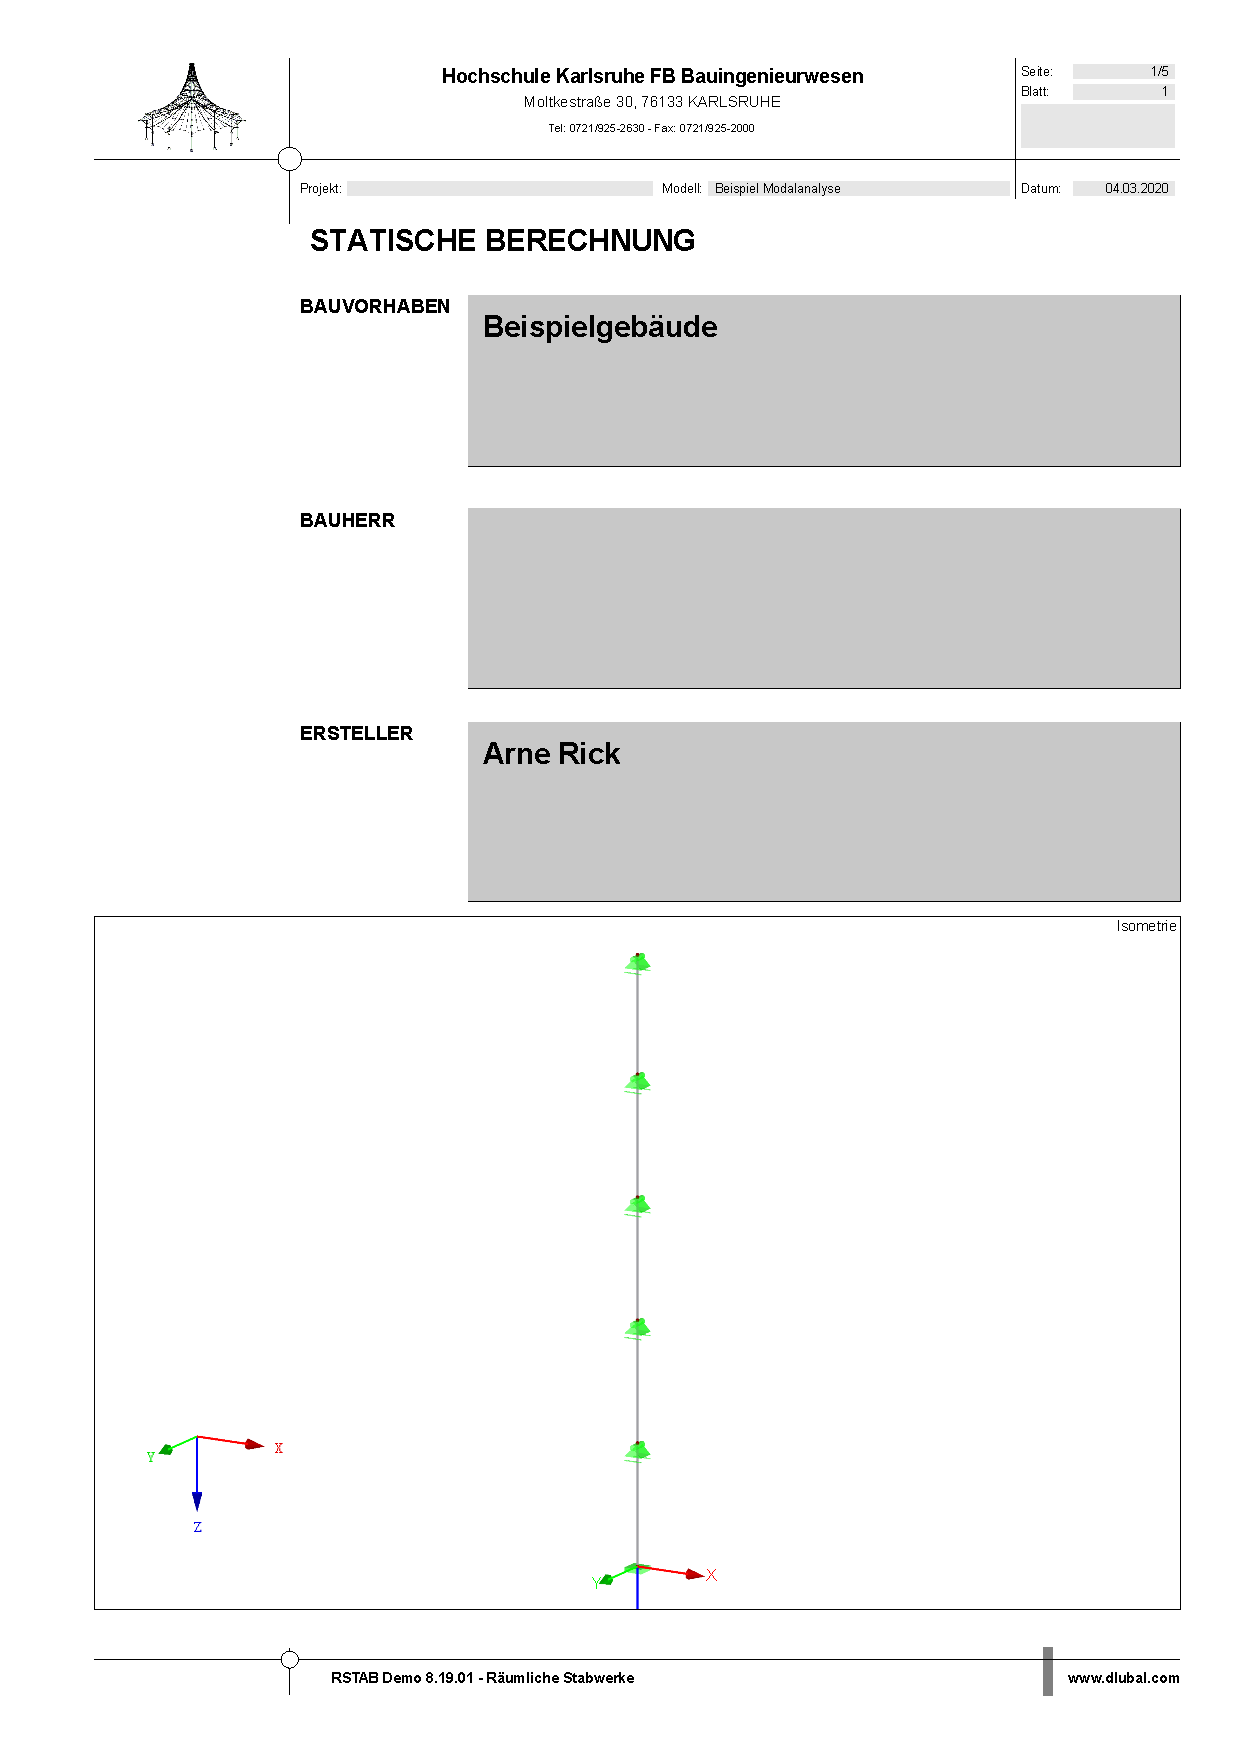
\includepdf[pages=-]{Ausdruckprotokoll_-_RStab.pdf}

